\documentclass[l3doc]{hduthesis}

\DocInfo
  {
    title        = The \hologo{hduthesis} Class\\
                   \hologo{LaTeX} Thesis Template for
                   Hangzhou Dianzi University,
    author       = Mingyu Xia \mailto{xiamyphys@hdu.edu.cn}
                   \footnote{Physics Department, Graduate in 06/2025},
    CJKmain-font = {[AutoFakeSlant]{Songti SC}},
    CJKsans-font = {[BoldFont = Hei, AutoFakeSlant]{Heiti SC}},
    CJKmono-font = {[AutoFakeSlant]{LXGW WenKai Mono}}
  }

\begin{document}

\maketitle

\begin{abstract}
  \hologo{hduthesis} 是杭州电子科技大学学位论文 \hologo{LaTeX} 模板,支持学士、硕士学位论文排版.
\end{abstract}

\begin{center}
  \small\bfseries User Agreement
\end{center}
\begin{enumerate}\small
  \item 本模板通过 LPPL 1.3c 协议开放源代码,您可以随意使用编译出的 PDF 文件.
  \item 本模板根据杭州电子科技大学教务处颁发的 \href{https://jwc.hdu.edu.cn/2022/0428/c4528a153813/page.htm}{杭电理工类毕业论文写作规范} 编写而成,作者不对使用本模板产生的格式审查问题负责. \emph{如果您所在的学院因论文查重、收录等原因要求提交 \file{.docx} 格式,不接收 \file{.pdf} 论文稿件,请勿执意使用本模板,避免因格式转换带来不必要的麻烦.} 使用本模板时,请按编译错误提示操作来勾选同意用户协议.
  \item 欢迎前往 GitHub 提交反馈意见,为推动学校认证与规范化 \hologo{hduthesis} 贡献力量.
\end{enumerate}
\endtitlepage
\restoregeometry

\section{Introduction \& Loading \hologo{hduthesis}}

本模板为杭州电子科技大学学位论文 \underline{非官方} \hologo{LaTeX} 模板,
以 \hologo{LaTeX3} 构建,支持学士和硕士学位论文排版.
加载 \hologo{hduthesis} 时遇到``编译受阻''报错,请认真阅读上页的用户协议.
键入全局选项 \cmd{agreed} 后,方可顺利进行编译,并默认您已同意用户协议.

\begin{framed}
  \begin{verbatim}
    \documentclass [ agreed, ... ] { hduthesis }
  \end{verbatim}
\end{framed}

\section{Generate the Cover}

\begin{function}{\DocInfo}
  \begin{syntax}
    \cs{DocInfo}\marg{keyvals}
  \end{syntax}

  此命令接收键值,用于设置文档信息. 键 \keys{\cmdmac~title} 用于设置论文标题,键 \keys{\cmdmac~department} 用于设置学院,键 \keys{\cmdmac~major} 用于设置专业,键 \keys{\cmdmac~class} 用于设置班级,键 \keys{\cmdmac~stdntid} 用于设置学号,键 \keys{\cmdmac~author} 用于设置作者,键 \keys{\cmdmac~supervisor} 用于设置导师,键 \keys{\cmdmac~bibsource} 用于设置插入参考文献文件源. 命令会根据输入的学号自动判断使用者为本科生/研究生.

  命令 \cs{DocInfo} 需在导言区中执行. 完成文档信息输入后,在 \verb|\begin{document}| 后执行命令 \cs{maketitle} 会调用所设置的键值自动生成 \emph{论文封面} 和 \emph{诚信承诺书}.
\end{function}

本科生输入样例如下. 需要使用键 \keys{\cmdmac~title} 设置类型为毕业设计/毕业论文,使用斜线 (/) 分隔,如 \cmd{title = 杭州电子科技大学学位论文 \hologo{LaTeX} 模板/毕业论文}.

\begin{framed}
  \begin{verbatim}
    \DocInfo
      {
        title      = 杭州电子科技大学学位论文 \hologo{LaTeX} 模板/毕业论文,
        department = 理学院, major      = 物理学, stdntid   = 21668668,
        author     = 申智能, supervisor = 李智能, bibsource = reference
      }
  \end{verbatim}
\end{framed}

下页的缩略图为本科毕业论文文档样例 \cmd{hduthesis-bc} 中的封面、扉页和承诺书.

\includepdfmerge
  [ angle = -90, nup = 1x2, frame, linktodoc, scale = 0.96, delta = 0 .25in ]
  { /Users/xiamyphys/Desktop/LaTeXer/hduthesis/examples/hduthesis-bc.pdf, 1-2 }

研究生输入样例如下. 硕士学位论文扉页需同时有英文版,因此需要在键 \keys{\cmdmac~title} \keys{\cmdmac~author} \keys{\cmdmac~supervisor} 中分别输入中文和英文信息,中英信息使用斜线 (\cmd/) 分隔. 如作者中文姓名为 \cmd{申智能},英文姓名为 \cmd{SAN Chi Nan},则键值输入格式为 \cmd{author = 申智能/SAN Chi Nan}. 指导教师职称和姓名之间用半角冒号 (\cmd:) 分隔.

\begin{framed}
  \begin{verbatim}
    \documentclass { hduthesis }
    \DocInfo
      {
        title      = 杭州电子科技大学学位论文 \hologo{LaTeX} 模板/
                     \hologo{LaTeX} Template for Thesis at
                     Hangzhou Dianzi University,
        major      = 物理学,             stdntid    = 216686680,
        author     = 申智能/SAN Chi Nan, bibsource  = reference
        supervisor = 教授:葉芷晴/Prof.:YIP Tsz Ching,
      }
    \begin{document}  \maketitle  ...  \end{document}
  \end{verbatim}
\end{framed}

\DescribeMacro{\l__hduthesis_grade_int}
论文完成日期和学生毕业年份会根据当前系统时间自动生成. 如果当前月份在8月及以前,毕业年份会显示今年;如果当前月份在9月及以后,毕业年份会显示次年. 在 \cs{DocInfo} 后对整型 \cs{l__hduthesis_grade_int} 重新赋值可手动更改毕业年份.

\begin{verbatim}
  \ExplSyntaxOn  \int_set:Nn \l__hduthesis_grade_int <Year>  \ExplSyntaxOff
\end{verbatim}

下页包含所生成的硕士学位论文封面、扉页和承诺书缩略图. 此文档样例可在终端执行 \cmd{texdoc hduthesis-pg} 获取.

文档类同时提供了校徽 (\file{hdulogo.pdf})、校名 (\file{hdutitle.pdf}) 、校训 (\file{hdumotto.pdf})和校牌 (\file{hdubadge.pdf}) 的矢量素材,可直接使用. 以上文件均由 \href{https://www.hdu.edu.cn/666/list.htm}{校情纵览/校标规范} 所提供素材裁切制成,均支持在 \hologo{XeLaTeX} 和 \hologo{pdfLaTeX} 编译器下使用 \pkg{Ti\textit k\/Z} 等方式设置透明度.

\includepdfmerge
  [ nup = 2x2, frame, linktodoc, scale = 0.96, delta = .25in .25in ]
  { /Users/xiamyphys/Desktop/LaTeXer/hduthesis/examples/hduthesis-pg.pdf, 1-8 }

\section{Enter Abstract in EN / CN}

\DescribeEnv{abstract}
环境 \env{abstract} 用于生成摘要,其可选参数可设置语言格式.

\DescribeMacro{\keywords}
命令 \cs{keywords} 需在 \env{abstract} 环境内执行,其会根据 \env{abstract} 环境所选择的语言,自动生成英文 / 中文格式的关键词.

\begin{framed}
  \begin{verbatim}
    \begin{abstract}[en]...\keywords{keyword1, keyword2}  \end{abstract}
    \begin{abstract}[cn]...\keywords{关键词1, 关键词2}   \end{abstract}
  \end{verbatim}
\end{framed}

通过命令 \cs{keywords} 以半角逗号 (,) 为分隔输入关键词列表,输出时会根据所处 \env{abstract} 环境选择的语言不同,自动以半 / 全角分号分隔. 下图为生成的中/英摘要样例,可在终端执行 \cmd{texdoc hduthesis-bc} 获取此样例文件.

\begin{figure}[htbp]
  \centering
  \fbox
  {
    \includegraphics[page = 3, width = .42\linewidth]
    {/Users/xiamyphys/Desktop/LaTeXer/hduthesis/examples/hduthesis-bc.pdf} }
  \hfill
  \fbox
  {
    \includegraphics[page = 4, width = .42\linewidth]
    {/Users/xiamyphys/Desktop/LaTeXer/hduthesis/examples/hduthesis-bc.pdf} }
  \caption{样例文件 \file{hduthesis-bc.pdf}, Page 3 -- 4}
\end{figure}

\section{Input Text}

\hologo{hduthesis} 的 {chapter}、\cs{section}、\cs{subsection}、\cs{enumerate} 等段落级次均已按``\href{https://jwc.hdu.edu.cn/2022/0428/c4528a153813/page.htm}{杭电理工类毕业论文写作规范}''定制,可直接使用.

如需插入参考文献,通过命令 \cs{DocInfo} 指定 \file{.bib} 文件后在要插入参考文献等地方输入 \cs{printbiblography} 即可输出参考文献列表. 参考文献格式已设置为 \cmd{gb7714-2015}. 若未指定参考文献 \file{.bib} 文件,为加速编译,\pkg{gbt7714} 宏包将不会加载. 同时,模板额外预置了以下宏包

\begin{table}[htbp]
  \centering
  \begin{tabular}{*{8}{>{\small}p{.096\linewidth}}}
    \toprule
    \pkg{amsmath}    & \pkg{amssymb}   & \pkg{bm}         & \pkg{booktabs} &
    \pkg{cancel}     & \pkg{circuitikz}& \pkg{cleveref}   & \pkg{derivative} \\
    \midrule
    \pkg{extarrows}  & \pkg{fixdif}    & \pkg{listings}   & \pkg{mathtools}  & \pkg{multicol}   & \pkg{pgfplots}  & \pkg{physics2}   & \pkg{siunitx}\\
    \bottomrule
  \end{tabular}
\end{table}

\begin{figure}[htbp]
  \begin{subfigure}{.32\linewidth}
    \centering
    \fbox
    {
      \includegraphics[page = 5, width = .9\linewidth]
      {/Users/xiamyphys/Desktop/LaTeXer/hduthesis/examples/hduthesis-bc.pdf}
    }
    \caption{Table of Contents}
  \end{subfigure}
  \hfill
  \begin{subfigure}{.32\linewidth}
    \centering
    \fbox
    {
      \includegraphics[page = 11, width = .9\linewidth]
      {/Users/xiamyphys/Desktop/LaTeXer/hduthesis/examples/hduthesis-bc.pdf}
    }
    \caption{Text}
  \end{subfigure}
  \hfill
  \begin{subfigure}{.32\linewidth}
    \centering
    \fbox
    {
      \includegraphics[page = 12, width = .9\linewidth]
      {/Users/xiamyphys/Desktop/LaTeXer/hduthesis/examples/hduthesis-bc.pdf}
    }
    \caption{Text with figures}
  \end{subfigure}
\end{figure}

\hrule

\begin{center}
  \fbox
    { \parbox[c][1.5em]{34ex}{\centering\file{hduthesis-pg.config-module}} }
  \fbox { \parbox[c][1.5em]{32ex}{\centering\file{hduthesis-typeset-module}} }
  \fbox { \parbox[c][1.5em]{15ex}{\centering\file{hdulogo.pdf}} }\\[2ex]
  \fbox { \parbox[c][1.5em]{33ex}{\centering\file{hduthesis-bc.config-module}} }
  \qquad \fbox { \parbox[c][1.5em]{16ex}{\centering\file{hdubadge.pdf}} } \qquad
  \fbox { \parbox[c][1.5em]{16ex}{\centering\file{hdumotto.pdf}} }\\[2ex]
  \fbox { \parbox[c][1.5em]{30ex}{\centering\file{hduthesis-layout-module}} }~
  \fbox { \parbox[c][1.5em]{16ex}{\centering\file{hdutitle.pdf}} }
  \fbox
    { \parbox[c][1.5em]{34ex}{\centering\file{hduthesis-stationery-module}} }~
\end{center}

\hrule

\section{杭州电子科技大学信纸}

加载全局选项 \pkg{stationery},并进行文档信息设置,即可生成信纸. 可用于推荐信撰写.
此模块无需 \pkg{agreed} 选项.

\begin{framed}
  \begin{verbatim}
    \documentclass [ stationery ] { hduthesis }
  \end{verbatim}
\end{framed}

与学士 / 硕士学位论文文档信息设置类型,使用 \cs{DocInfo} 命令,对信件标题、发件人、机构、日期、电话和邮件信息进行设置. 此时 \cs{DocInfo} 命令接受键
\keys{\cmdmac~title} \keys{\cmdmac~author} \keys{\cmdmac~affliction}
\keys{\cmdmac~date} \keys{\cmdmac~tel} \keys{\cmdmac~mail}. 下页为生成信纸的样例.

\begin{framed}
  \begin{verbatim}
    \DocInfo
      {
        title      = Recommendation Letter for SAN Chi Nan,
        author     =  YIP Tsz Ching,
        affliction = {Physics Department, Hangzhou Dianzi University},
        date       = {25\textsuperscript{th} November, 2024},
        tel        = (852) 3141-5926,
        mail       = xiamyphys@gmail.com
      }
  \end{verbatim}
\end{framed}

\section{For Developers}

本手册为 \cls{hduthesis} 加载选项 \pkg{l3doc} 后生成,基于 \cls{l3doc} 文档类.

\begin{framed}
  \begin{verbatim}
    \documentclass [ l3doc ] { hduthesis }
  \end{verbatim}
\end{framed}

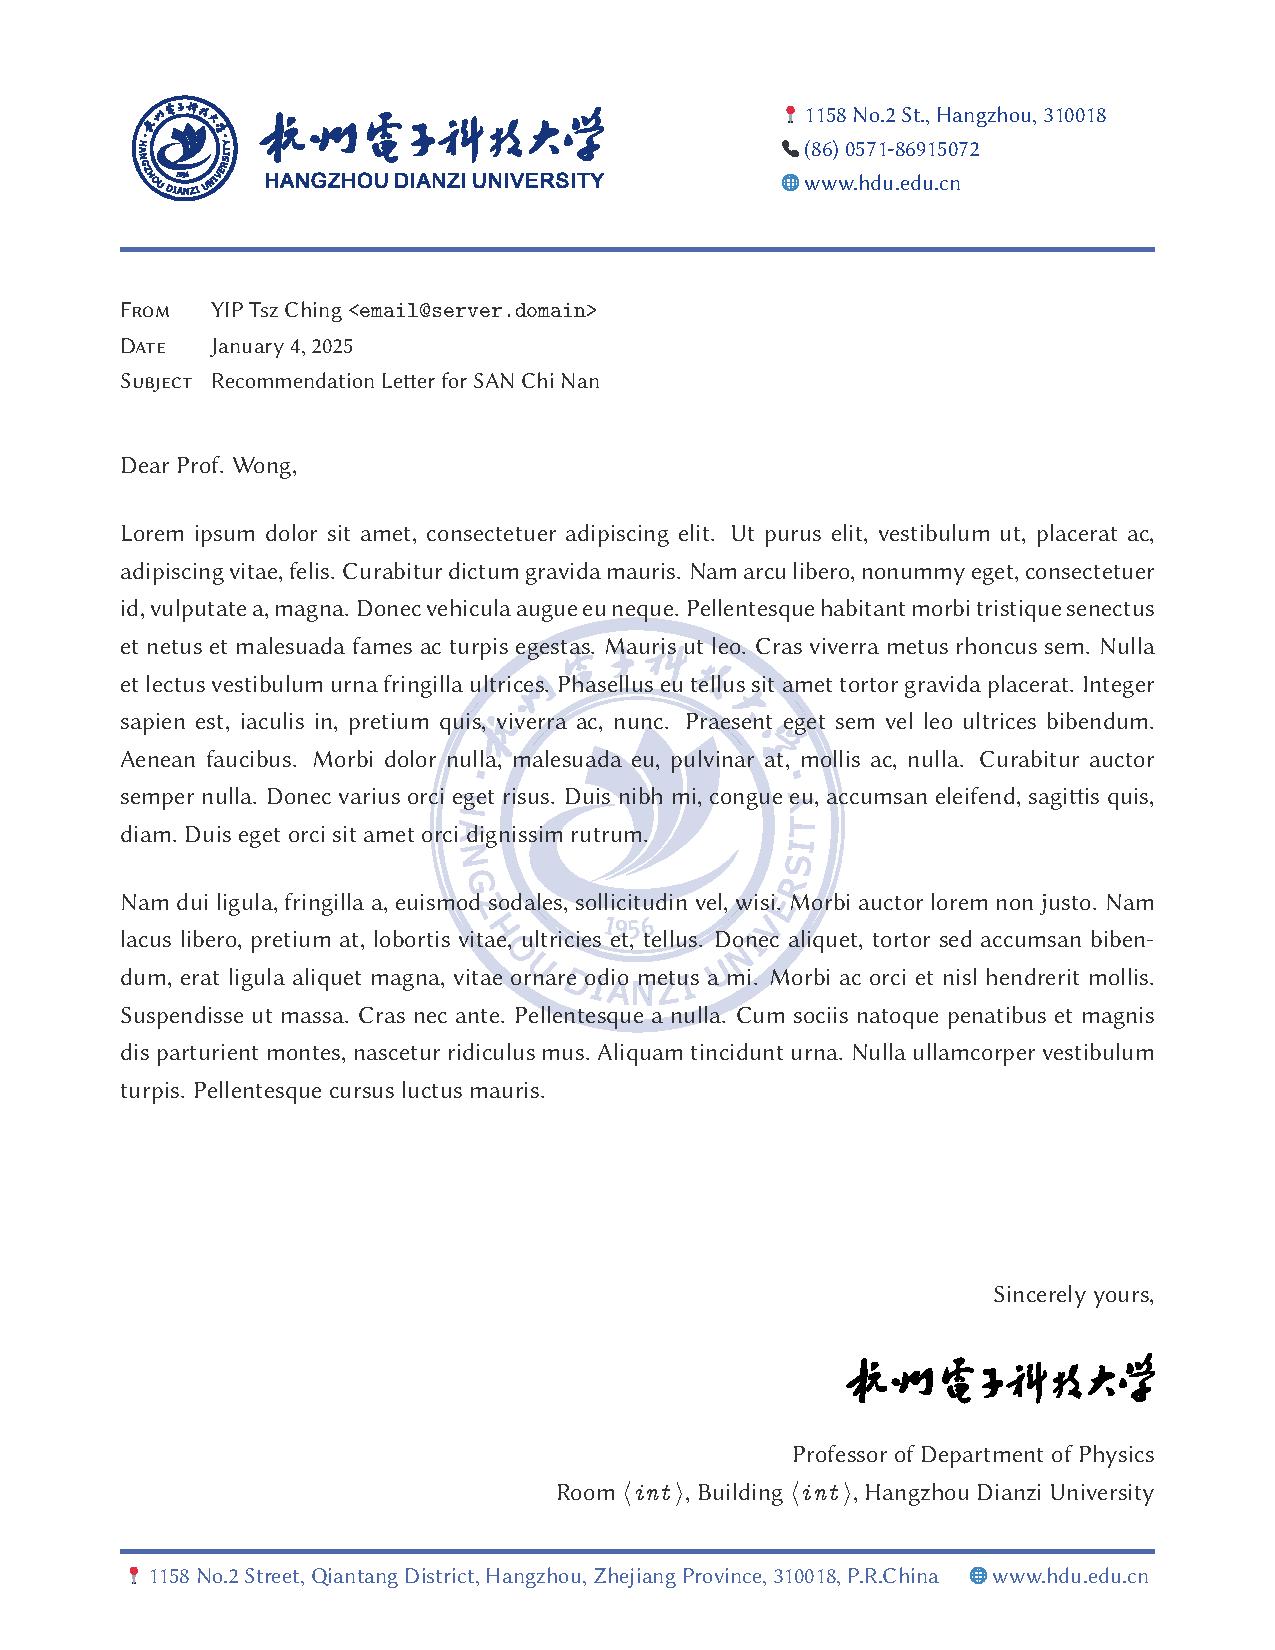
\includepdf{/Users/xiamyphys/Desktop/LaTeXer/hduthesis/examples/hduthesis-stationery}

\end{document}
